\section{Software Testing and Test Validity}

Architectural drift, discussed above, concerns whether generated code stays structurally consistent with the rest of a project over time. This section addresses a related but distinct question, one that applies even to a single, well-isolated piece of code: when a test passes, how much does that actually tell us?

\textbf{A passing test versus a valid test.} A test passing means only one specific thing: the code, when run against that particular test, produced the outcome the test checked for. It says nothing about whether the test checked for the right thing in the first place. A test suite can run to completion, report every test as passing, and even claim high coverage of the codebase, while still failing to verify that the software does what it was actually supposed to do --- because the tests themselves never asked the right question. This gap, between a test passing and a test validating the intended behavior, is the central concern of this section.

\textbf{Why this gap is particularly relevant when tests are agent-generated.} As established earlier, an LLM has no inherent mechanism for verifying its own output against anything beyond what it was given --- it can produce plausible, syntactically correct output, but has no independent way of confirming that output is actually right. A generated test is not exempt from this limitation; it is itself just another piece of generated code, subject to the same constraint. An agent asked to "write tests for this feature" can produce a test suite that runs successfully and reports strong coverage numbers, while the tests themselves check only shallow properties of the code rather than its intended behavior. This is not a hypothetical risk: the literature has found that code coverage is weakly correlated with the effectiveness of LLM-generated tests in detecting bugs, meaning a test suite can exercise a large portion of the code without being any good at catching cases where that code is wrong.

\begin{figure}[H]
    \centering
    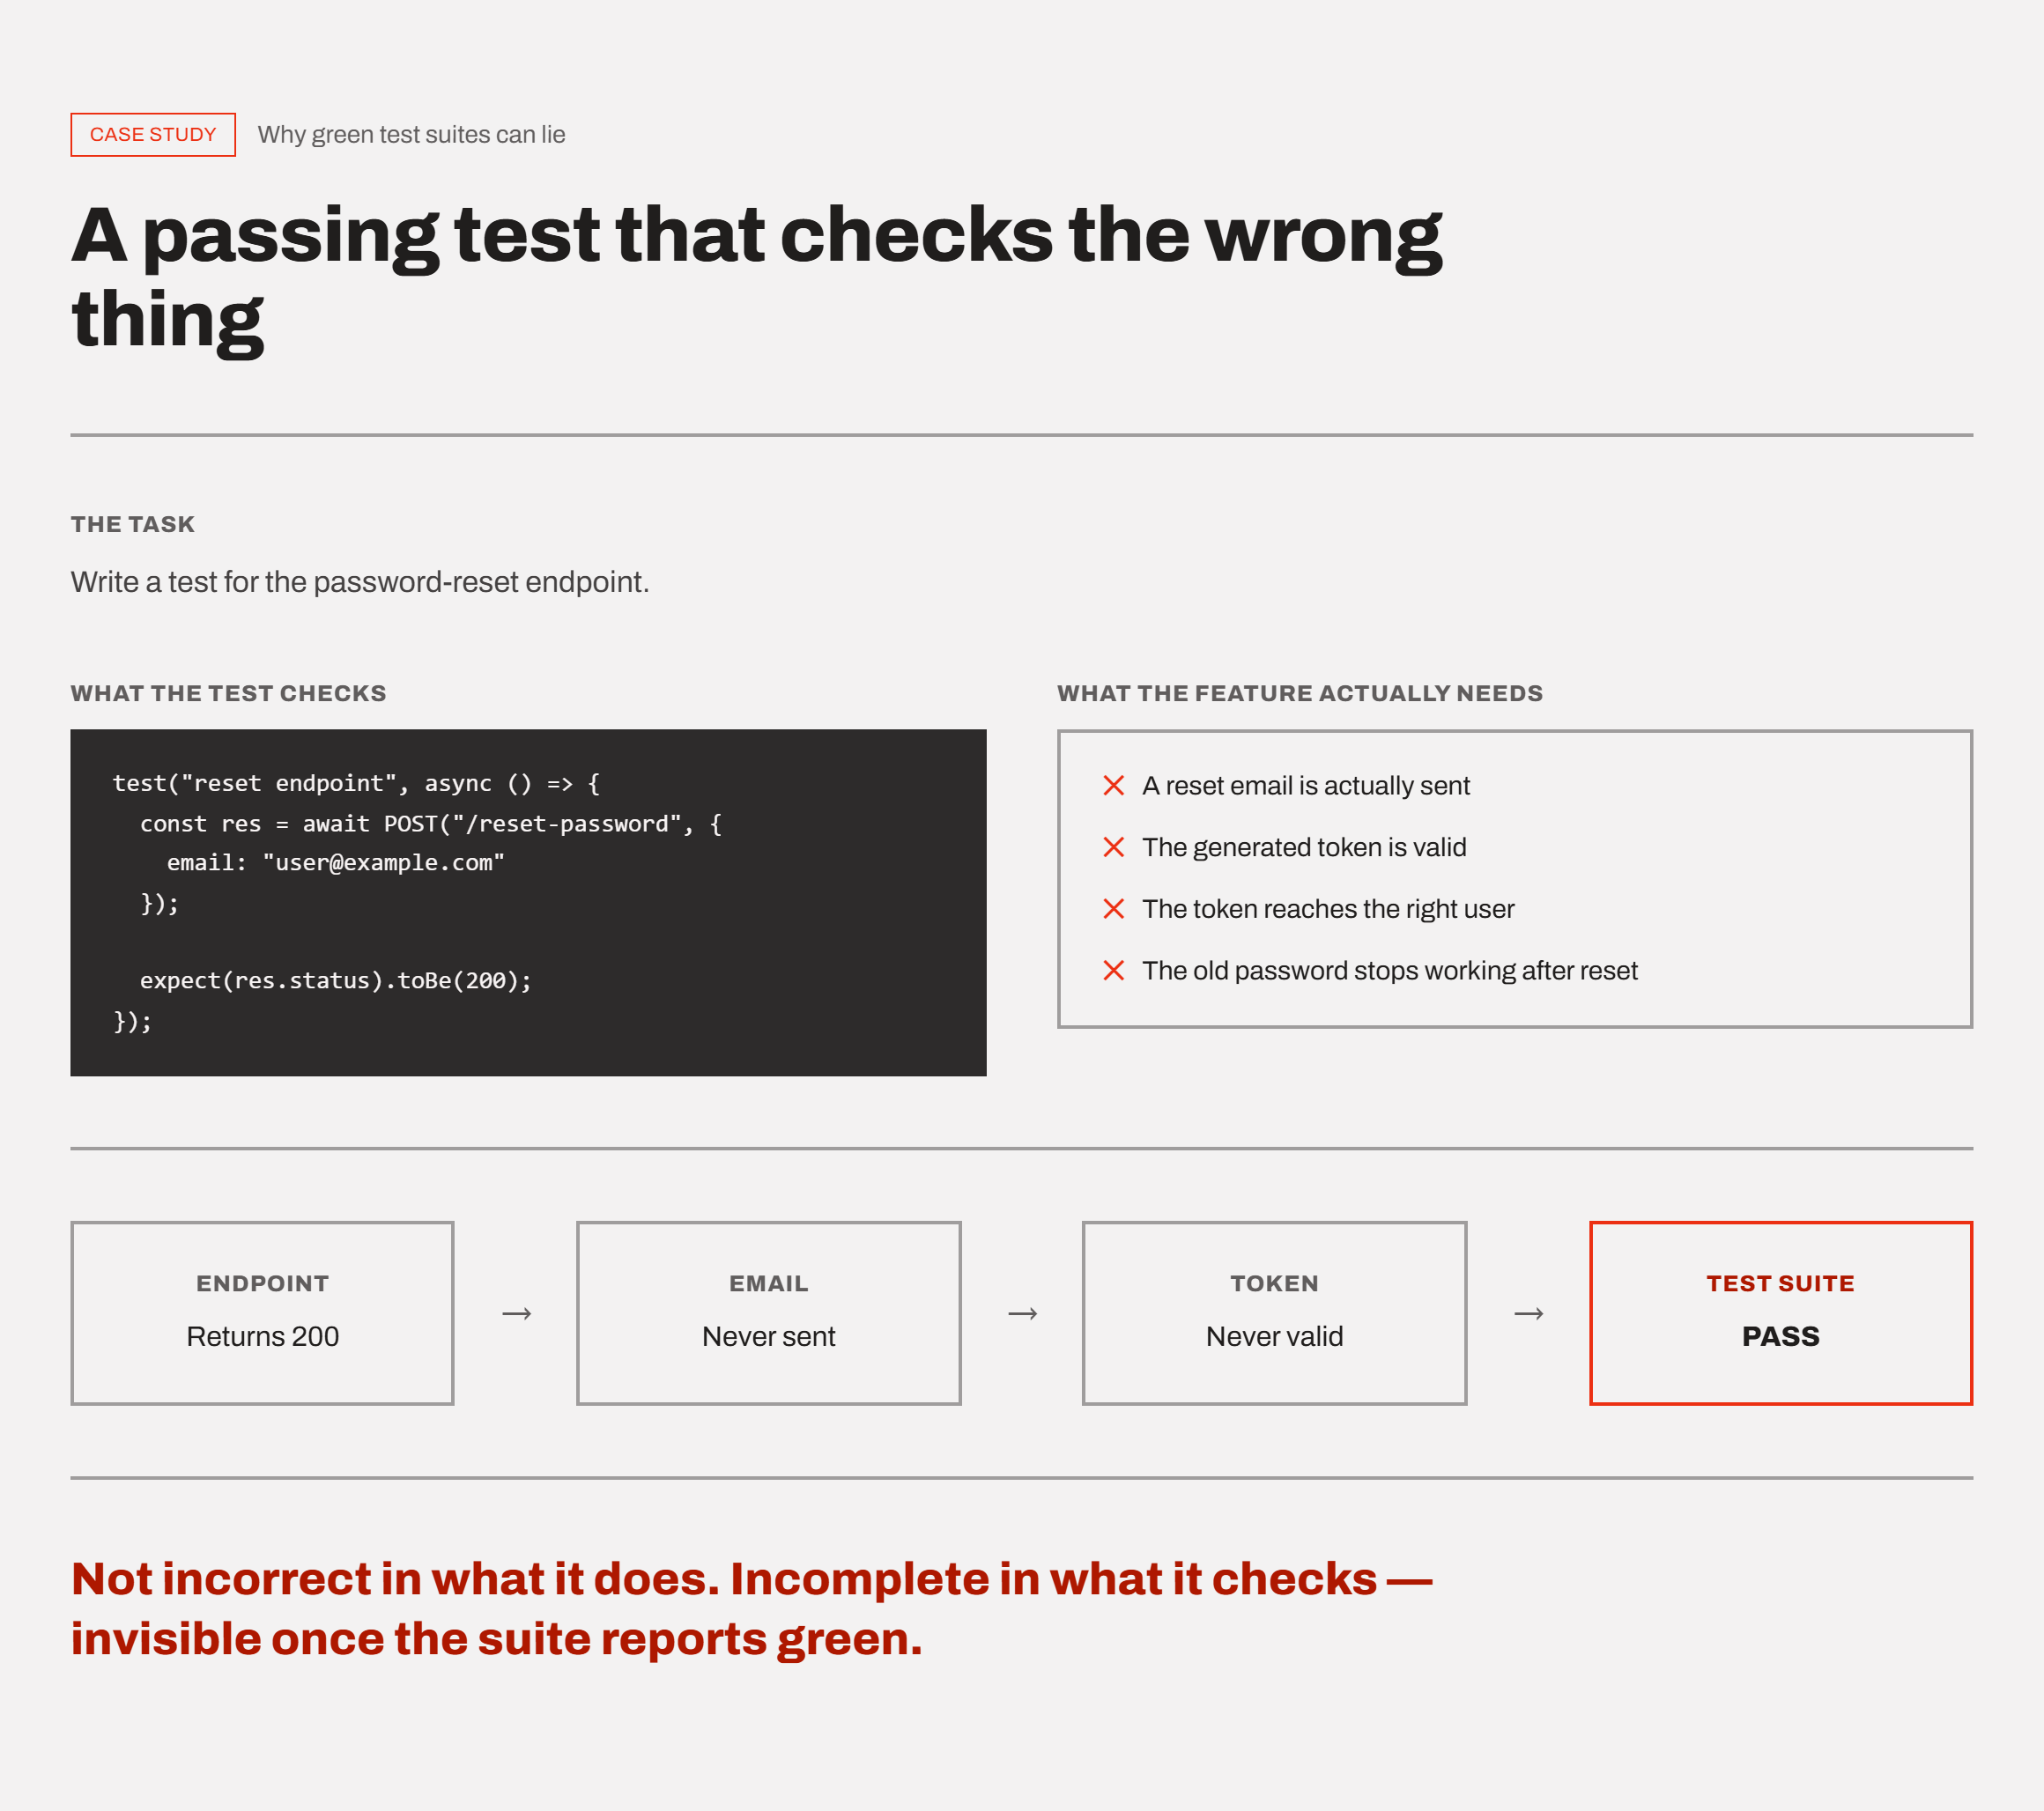
\includegraphics[width=\linewidth]{Bilder/Foundations/test-validity.png}
    \caption{A passing test suite versus a test suite that actually validates the intended behavior.}
    \label{fig:test-validity}
\end{figure}

\textbf{A concrete illustration.} Consider an agent asked to write tests for a password-reset endpoint. A test that only checks that calling the endpoint returns a successful HTTP status code will pass regardless of whether a reset email was actually sent, whether the generated token is valid, or whether the token even reaches the right user --- the endpoint could be broken in exactly the way that matters to the feature's purpose, and this test would still report success. The test is not incorrect in what it does; it is incomplete in what it checks, and that incompleteness is invisible from the outside once the test suite reports green.

\textbf{A related but distinct failure mode: tests that validate the implementation rather than the requirement.} A separate risk arises when the same agent, or the same generation process, produces both the implementation and its tests. In this situation, a test can end up confirming that the code behaves the way the code happens to behave, rather than the way the original requirement intended. Empirical work on LLM-based test generation has documented this concretely: when a model is prompted with a buggy implementation, it can treat the faulty behavior as intended and generate a test that asserts the incorrect outcome, rather than the behavior the function was actually supposed to have --- the resulting test still passes, and still contributes to coverage, while actively encoding the wrong behavior as if it were correct. This is a different problem from incomplete coverage: the test is not merely checking too little, it is checking the implementation against itself rather than against the original, independent requirement it was meant to satisfy.

Taken together, these observations point to the same underlying principle: whether a test suite is any good cannot be judged from whether it passes, or even from how much of the code it exercises, but only by checking it against the original requirement the software was meant to fulfill --- a check the test suite itself, by construction, cannot perform on its own behalf.

